% !Mode:: "TeX:UTF-8"
\documentclass[final]{jcr}

\usepackage[linesnumbered,ruled]{algorithm2e}
\usepackage{bm}
\usepackage{lastpage}
\usepackage{enumitem}
\usepackage{booktabs}
\usepackage{longtable}
\hypersetup{hidelinks}

\makeatletter
\def\jcr@date@year{}
\def\jcr@date@month{0}
\def\jcr@page@start{}
\def\jcr@page@end{}
\makeatother

\begin{document}

% 课程报告不使用期刊 DOI、卷期、收稿日期、定稿日期和页码范围等字段。
\setcounter{page}{1}
\AuthorCiteInput{ZENG J Q}

\CLCnumber{TP309.7}

\begin{frontmatter}
  \title{基于秘密共享的密态异常梯度过滤与鲁棒安全聚合机制研究}
  \etitle{Privacy-Preserving Robust Federated Aggregation Against Label-Flipping and Byzantine Attacks via Secret-Shared Similarity Filtering}

  \author[1]{曾嘉祺}
  \eauthor[1]{ZENG Jia-Qi}

  \address[1]{广东外语外贸大学 信息科学与技术学院（网络空间安全学院）, 广州 510006; E-mail: 20251010015@mail.gdufs.edu.cn}
  \eaddress[1]{School of Information Science and Technology, Guangdong University of Foreign Studies, Guangzhou 510006, China; E-mail: 20251010015@mail.gdufs.edu.cn}

  \begin{abstract}
联邦学习同时面临模型更新泄露和恶意客户端投毒风险。安全聚合能够隐藏单个更新，却无法在聚合前识别异常；Krum 等鲁棒方法可以过滤拜占庭更新，却通常要求服务器访问明文梯度。本文提出课程原型 PP-SRSF：客户端将高维更新压缩为随机投影草图，定点量化并加性秘密共享；两个非共谋聚合方使用 Beaver triple 计算草图平方距离，再对保留更新执行成对掩码安全聚合。实验覆盖 MNIST、Fashion-MNIST、三类攻击、三随机种子及最高 60\% 恶意比例，并与 FedAvg、明文鲁棒方法和 FedGT 组测试基线比较。结果表明，PP-SRSF 对符号翻转和高斯噪声保持稳定；三随机种子标签翻转下 PP-SRSF、Trust 扩展与论文对齐的 FedGT-$\hat n_m$ 适配基线准确率分别为 $0.602\pm0.058$、$0.611\pm0.077$ 与 $0.662\pm0.079$。同时，成对标签翻转和多数标签投毒仍会削弱距离过滤，体现了隐私、鲁棒性与效率之间的边界。
  \end{abstract}

  \begin{keywords}
联邦学习; 安全聚合; 秘密共享; 拜占庭鲁棒性; 标签翻转攻击; 多方安全计算
  \end{keywords}

  \begin{eabstract}
Federated learning faces both update leakage and malicious-client poisoning. This report proposes PP-SRSF, a course-level prototype that compresses updates into random-projection sketches, additively secret-shares them, evaluates squared distances with Beaver triples, and aggregates selected updates with pairwise masks. Experiments cover MNIST, Fashion-MNIST, three attacks, three random seeds, and up to 60\% malicious clients. PP-SRSF remains effective against sign-flipping and Gaussian noise, while label-flipping and majority poisoning expose the limits of distance-only filtering. A history/trust extension and a paper-aligned FedGT-$\hat n_m$ adaptation provide stronger recent baselines without being presented as full malicious-secure MPC.
  \end{eabstract}

  \begin{ekeywords}
federated learning; secure aggregation; secret sharing; Byzantine robustness; label-flipping attack; secure multi-party computation
  \end{ekeywords}
\end{frontmatter}

\zihao{-5}

\section{引言}
联邦学习允许多个客户端在不直接共享原始数据的情况下协同训练模型，但客户端上传的梯度或模型更新仍可能泄露本地数据分布、成员信息和敏感特征。同时，恶意客户端可以通过标签翻转、符号翻转或高斯噪声更新破坏全局模型收敛。现有安全聚合协议以 Bonawitz 等人的 SecAgg 为代表，主要解决服务器无法看到单个明文更新的问题\cite{bonawitz2017secagg}；现有鲁棒聚合算法则以 Krum、坐标截断均值和坐标中位数为代表，主要依赖明文更新之间的距离或坐标统计\cite{blanchard2017krum}。这导致隐私保护和鲁棒过滤之间存在结构性矛盾：如果服务器看不到单个更新，就难以判断哪些更新异常；如果服务器能够执行明文异常检测，客户端更新隐私又会被削弱。

近三年的研究开始关注可验证安全聚合、隐私保护鲁棒联邦学习和多数恶意客户端鲁棒性。例如 Sophon 通过双重信任机制提升拜占庭鲁棒性\cite{sophon2025}，DP-BREM 与可验证差分隐私方案同时考虑隐私和拜占庭鲁棒\cite{gu2025dpbrem,zhang2025verifiabledp}，FedAMM 关注多数恶意客户端下的鲁棒聚合\cite{fedamm2025}，可验证多轮安全联邦学习则强调 dropout、效率和聚合正确性\cite{li2026verifiable}。这些工作说明，仅讨论模型准确率已经不足以满足现代密码学课程中“AI + 密码”交叉问题的要求，必须同时分析系统模型、威胁模型、密码学原语、协议交互和实验可复现性。

基于上述矛盾，本文围绕三个研究问题展开：低维随机投影能否保留足以识别强异常更新的距离结构；秘密共享与 Beaver 乘法能否在不公开单个草图的条件下完成过滤；该折中在不同攻击、恶意比例和草图维度下具有怎样的精度、检测率与通信边界。本文的贡献是提出并实现 PP-SRSF 课程原型，给出半诚实双聚合方模型下的泄露与复杂度分析，并通过跨数据集、多攻击、多比例、多随机种子及协议微基准实验验证其有效范围和失败边界。

\section{相关工作}
\subsection{拜占庭鲁棒联邦学习}
Krum 首次系统化地将拜占庭容错思想引入分布式梯度聚合，通过选择与多数更新距离较近的更新来降低异常梯度影响\cite{blanchard2017krum}。后续工作进一步考虑数据异构、客户端动态性和多数恶意等真实场景。Zuo 等人研究了数据异构与拜占庭攻击并存时的鲁棒联邦学习\cite{zuo2025heterogeneity}；Sophon 使用辅助数据与双重信任机制应对任意数量恶意客户端\cite{sophon2025}；FedAMM 面向多数恶意客户端场景，强调在恶意比例超过半数时仍降低攻击成功率\cite{fedamm2025}。这些方法提高了鲁棒性，但往往依赖服务器对明文更新的统计分析。

从技术路线看，现有拜占庭鲁棒聚合大致可以分为三类。第一类是距离或相似度驱动的方法，以 Krum 及其变体为代表，假设诚实客户端更新在向量空间中形成较紧密的簇，而恶意更新会偏离该簇。这类方法直观且对符号翻转、高斯噪声等强异常更新有效，但在 Non-IID 数据下，诚实客户端之间也可能因为本地分布差异而距离较远，从而带来误杀风险。第二类是坐标统计鲁棒方法，如 Trimmed Mean、坐标中位数等，通过逐坐标裁剪极端值降低异常更新影响。该类方法计算开销较低，但忽略了不同参数坐标之间的相关性，对有方向性的协同投毒未必充分。第三类是信任、历史和辅助信息驱动的方法，例如 FLTrust 通过可信根数据估计更新方向可信度\cite{fltrust2021}，Sophon 进一步把辅助数据、双重信任和鲁棒聚合结合起来\cite{sophon2025}。这类方法通常更能处理隐蔽攻击，但需要额外可信数据或跨轮状态，系统假设更强。

2024--2026 年的相关研究趋势表明，鲁棒联邦学习的关注点正在从“少数粗暴拜占庭客户端”转向更复杂的现实约束：数据高度异构、恶意比例上升、攻击者具备自适应能力、训练存在客户端掉线，且鲁棒性与效率、隐私之间存在张力。Zuo 等人的工作强调 Non-IID 场景下鲁棒判断边界会被放大\cite{zuo2025heterogeneity}；FedAMM 关注多数恶意客户端下的模型聚合稳定性\cite{fedamm2025}；FedGT 与去中心化鲁棒联邦学习分别从安全聚合和双域聚类角度讨论恶意客户端识别\cite{fedgt2025,dfl2024dual}；ROBY、BPFLH 与不规则参与者场景下的鲁棒隐私联邦学习进一步说明，服务器less、异构数据和动态参与会让安全假设更复杂\cite{tang2025roby,zhu2026bpflh,chen2024irregular}。这些工作对本文有两点启发：其一，过滤规则不能只在理想 IID 假设下成立；其二，若要与安全聚合结合，过滤所需的统计量必须足够轻量，否则密态计算成本会抵消鲁棒收益。

\subsection{隐私保护与安全聚合}
安全聚合协议的目标是使服务器只能获得客户端更新总和，而无法恢复单个客户端更新\cite{bonawitz2017secagg}。近年研究进一步加入可验证性、dropout resilience 和轻量化设计，例如 Verifiable and Lightweight Multi-Round Secure Federated Learning\cite{li2026verifiable}、VPFLI\cite{ren2025vpfli} 以及公开验证的鲁棒 MPC 方案\cite{gai2025public}。这些工作与本文关注点互补：它们强调聚合正确性和隐私传输，而本文强调在安全聚合前加入隐私保护的异常过滤。

经典安全聚合的优势在于隐私边界清晰：服务器在协议结束时只获得整体和，单个客户端更新被掩码隐藏。但这种设计也造成结构性矛盾：服务器越看不到单个更新，越难判断哪些更新异常；若先公开更新做鲁棒过滤，隐私保护又失去意义。因此，安全聚合本身并不能自动提供鲁棒性。

近年的隐私保护联邦学习研究开始把安全聚合从“只隐藏更新”扩展到“隐藏更新同时支持附加判断”。VPFLI 强调隐私保护的联邦学习推理与身份机制\cite{ren2025vpfli}；Li 等人的多轮安全联邦学习协议关注可验证性和轻量化\cite{li2026verifiable}；Gai 等人的公开验证方案体现了 MPC 与聚合正确性验证结合的方向\cite{gai2025public}；移动云协同聚合提醒协议设计需考虑时延弹性和端侧资源约束\cite{tang2026mobilecloud}。这些工作说明，现代密码学工具可以为联邦学习提供比传输加密更细的安全性质。不过，将这些工具直接套到高维深度模型更新上通常代价较高，特别是密态距离、密态排序和密态中位数等操作需要大量乘法和比较。

\subsection{隐私与鲁棒性的联合优化}
DP-BREM 尝试同时实现差分隐私与拜占庭鲁棒性，通过客户端动量暴露跨轮累积的恶意扰动\cite{gu2025dpbrem}。Byzantine-Resilient Secure Aggregation for Federated Learning Without Privacy Compromises 则直接关注安全聚合与拜占庭鲁棒之间的矛盾\cite{xia2024secureagg}。压缩域鲁棒隐私联邦学习表明，在低维表示上完成鲁棒判断可以缓解高维密态计算成本\cite{hu2024compressive}。本文借鉴这一问题意识，但采用更轻量的随机投影草图作为过滤对象，避免在完整高维更新上执行昂贵的密态几何计算。

隐私与鲁棒性的联合优化难点在于二者天然拉扯。鲁棒聚合希望观察尽可能细的客户端级统计，以发现离群点、估计可信方向或裁剪极端坐标；隐私保护则希望最小化服务器或聚合方看到的客户端级信息。若完全偏向隐私，系统退化为普通安全聚合，面对投毒攻击缺乏预处理能力；若完全偏向鲁棒，系统又需要暴露明文更新或高维距离矩阵。Xia 等人的工作明确指出安全聚合与拜占庭鲁棒之间存在“不泄露单个更新”和“识别恶意更新”的功能冲突\cite{xia2024secureagg}。因此，本文选择的切入点不是宣称完全解决冲突，而是在泄露边界可说明、计算成本可运行的前提下，探索一种课程原型级折中。

与直接在密文域计算几何中位数或完整 Krum 相比，PP-SRSF 只把低维随机投影草图送入秘密共享协议。草图并非原始梯度，但保留了一部分距离结构，可作为异常检测的代理统计量。这样的设计牺牲了部分过滤精度，换来更低的密态计算与通信成本。垂直联邦学习中的表示学习方案也说明，异构场景下常需要用中间表示替代原始特征或梯度进行协作\cite{wang2025pravfed}。换言之，本文的贡献不在于提出一个工业级完整 MPC 协议，而在于把“鲁棒过滤所需的统计量”与“密码协议能够承受的输入规模”对齐，并通过实验展示这种折中在典型拜占庭攻击下具有可观察收益。

\section{系统模型与威胁模型}
\subsection{系统模型}
系统包含 $n$ 个客户端、一个联邦学习协调服务器和两个非共谋聚合方 $Agg_A,Agg_B$。第 $t$ 轮中，服务器广播全局模型 $w_t$，客户端 $i$ 在本地数据 $D_i$ 上训练得到更新 $\Delta_i$。客户端将 $\Delta_i$ 展平为向量 $x_i\in\mathbb{R}^{d}$，使用公开随机矩阵 $R\in\mathbb{R}^{m\times d}$ 生成草图
\[
s_i = R x_i,\quad m \ll d.
\]
之后客户端将 $s_i$ 定点量化为 $q_i=\lfloor S s_i\rceil\bmod p$，并生成加性秘密共享
\[
q_i^{(A)} + q_i^{(B)} \equiv q_i \pmod p.
\]
$Agg_A$ 和 $Agg_B$ 分别接收一份份额，并协同计算草图域距离或距离相关统计。服务器根据距离矩阵筛选客户端，再对筛选后的更新执行安全聚合。

\subsection{威胁模型}
本文采用课程实验级半诚实模型。聚合方遵循协议，但可能试图从收到的份额推断客户端草图；$Agg_A$ 与 $Agg_B$ 不共谋。客户端中存在比例为 $\rho$ 的恶意客户端，它们可以执行标签翻转、符号翻转或高斯噪声更新。服务器被视为诚实执行协调逻辑，但不应在过滤阶段获得完整明文更新。

需要强调的是，当前实现不是完整恶意安全 MPC。它不防止聚合方主动偏离协议、不处理复杂 dropout 恢复，也没有实现完全密文域几何中位数。本文将其定位为现代密码学课程原型，用于验证“秘密共享草图过滤 + 安全聚合”的系统可行性。

\begin{figure}
\centering
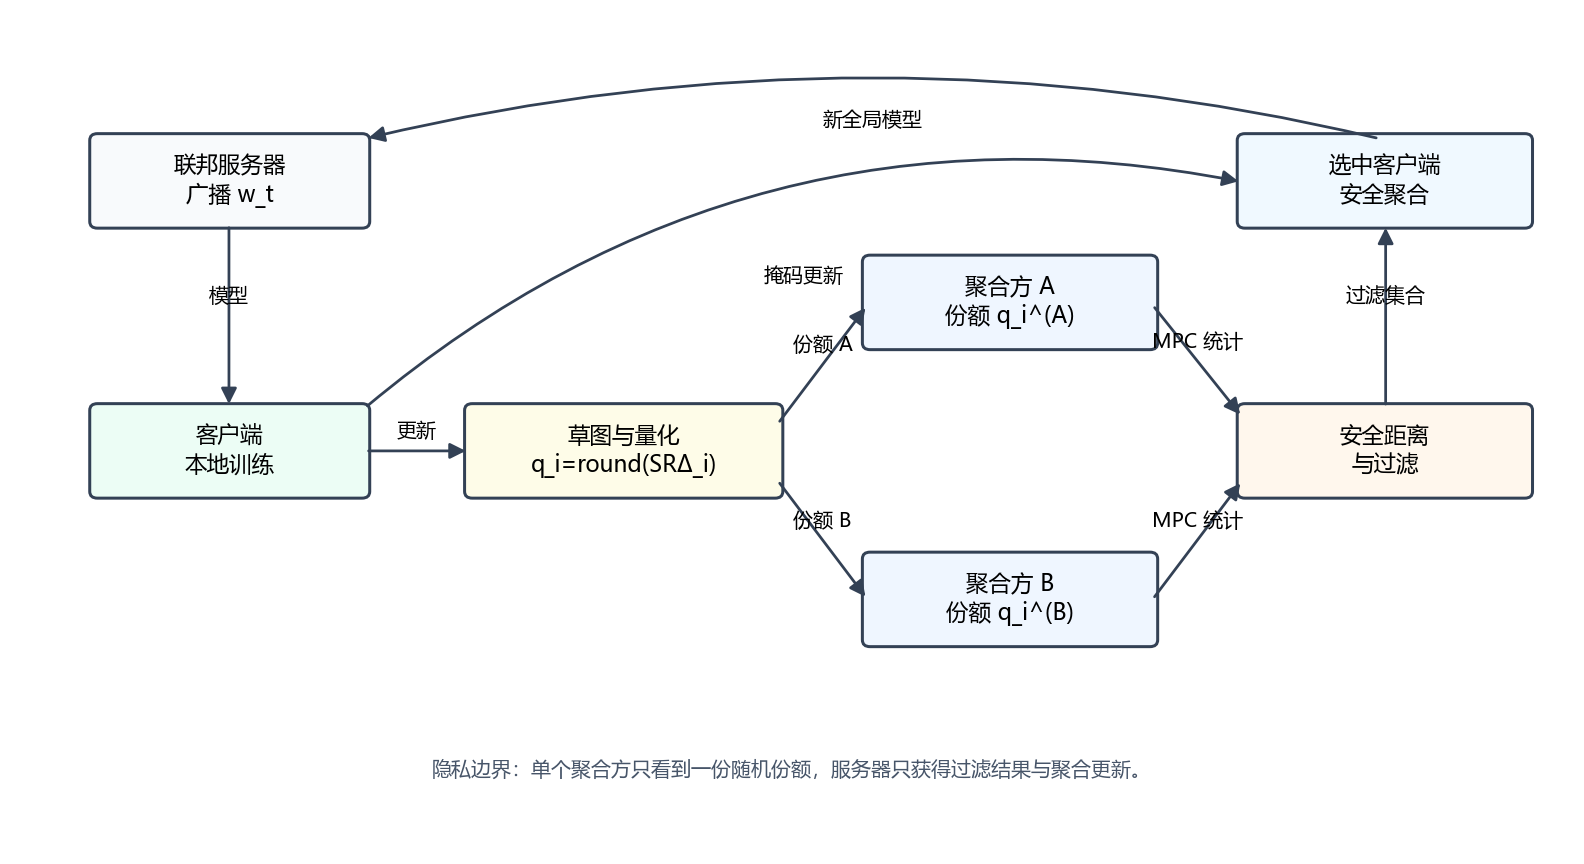
\includegraphics[width=0.95\linewidth]{../outputs/figures/protocol_architecture.png}
\caption{PP-SRSF 的系统交互与隐私边界}{}
\label{fig:protocol-architecture}
\end{figure}

图\ref{fig:protocol-architecture} 概括了本文协议流程。客户端本地训练后只把草图份额分别发送给两个聚合方；聚合方协同计算距离统计并返回过滤信息；服务器只对筛选后的掩码更新求和。该流程把“异常检测所需的相似度统计”和“完整模型更新”分开处理。

\begin{figure}
\centering
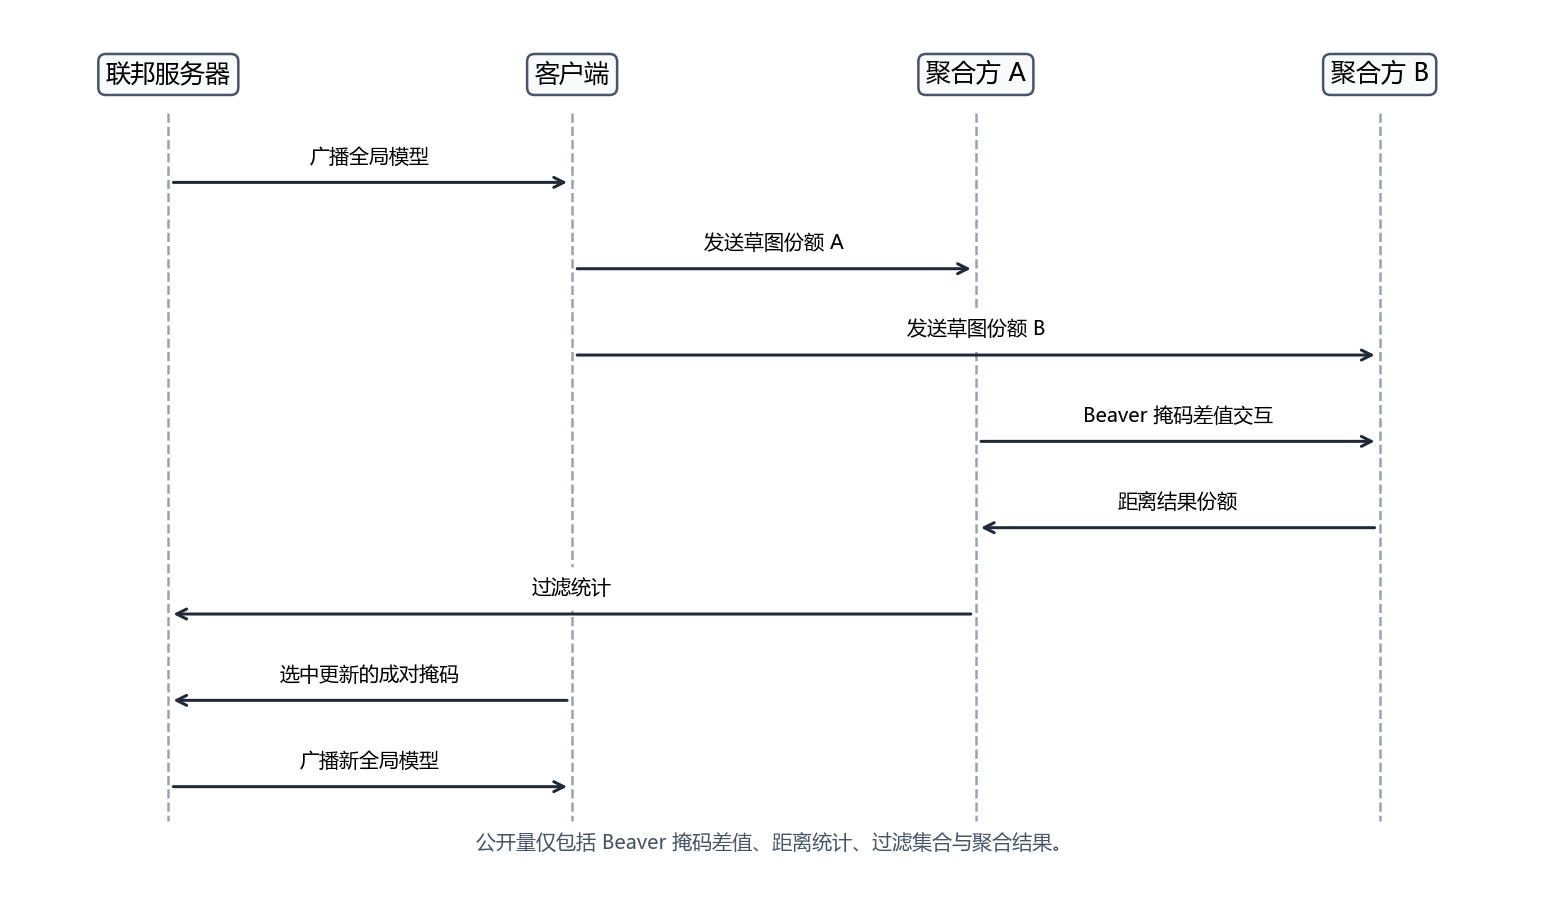
\includegraphics[width=0.95\linewidth]{../outputs/figures/protocol_sequence.png}
\caption{PP-SRSF 的协议时序与公开量}{}
\label{fig:protocol-sequence}
\end{figure}

图\ref{fig:protocol-sequence} 进一步给出一轮训练的消息顺序。两个聚合方只公开 Beaver 掩码差值和最终距离统计，服务器接收过滤集合与聚合结果，不接触单个草图或完整更新。

\section{PP-SRSF 方法设计}
\subsection{随机投影草图}
直接在高维模型更新上执行密态距离计算的成本为 $O(nd)$ 或 $O(n^2d)$。PP-SRSF 使用随机投影将更新降维到 $m$ 维，草图维度 $m$ 通常远小于模型参数维度 $d$。随机投影保留了异常更新与正常更新之间的相似性结构，同时显著降低后续秘密共享距离计算的输入规模。

\subsection{定点量化与加性秘密共享}
秘密共享通常在整数环或有限域上工作，因此需要将浮点草图转换为整数：
\[
q_{i,k}=\lfloor S\cdot s_{i,k}\rceil\bmod p.
\]
对每个坐标生成随机份额 $r_{i,k}$，令
\[
q_{i,k}^{(A)}=r_{i,k},\quad q_{i,k}^{(B)}=q_{i,k}-r_{i,k}\bmod p.
\]
单个聚合方仅持有随机份额，无法独立恢复 $q_i$。

\subsection{基于 Beaver triple 的平方距离}
对共享值 $x,y$，预处理阶段生成 $a,b,c=ab$ 的两方份额。在线阶段公开随机掩码差值 $e=x-a$ 与 $f=y-b$，并令
\[
z^{(A)}=c^{(A)}+eb^{(A)}+fa^{(A)}+ef,\quad
z^{(B)}=c^{(B)}+eb^{(B)}+fa^{(B)}.
\]
两份结果相加等于 $xy$。本文将该乘法逐坐标应用于 $q_i-q_j$，最后只重构距离 $D_{ij}$，不重构输入草图。当前 triple 由单进程可信预处理模拟生成，因而属于半诚实协议原型，不包含认证份额或恶意安全检查。

\subsection{草图域鲁棒过滤}
系统计算客户端间的平方欧氏距离
\[
D_{ij}=\|q_i-q_j\|_2^2.
\]
对每个客户端 $i$，使用 Krum 风格分数：
\[
score_i=\sum_{j\in N_i}D_{ij},
\]
其中 $N_i$ 是距离 $i$ 最近的 $n-f-2$ 个客户端集合，$f=\lfloor \rho n \rfloor$。系统保留分数最低的 $n-f$ 个客户端。

\renewcommand{\algorithmcfname}{算法}
\SetAlgoCaptionSeparator{~}
\begin{algorithm}[H]
  \zihao{6}
  \caption{\kaishu \zihao{-5} PP-SRSF 鲁棒安全聚合流程}
  \label{alg:ppsrsf}
  \LinesNumbered
  \KwIn{客户端集合 $C$，全局模型 $w_t$，草图维度 $m$，恶意客户端估计 $f$}
  \KwOut{新全局模型 $w_{t+1}$}
  \For{每个客户端 $i\in C$}{
    本地训练并得到模型更新 $\Delta_i$\;
    计算草图 $s_i=R\Delta_i$\;
    定点量化 $q_i=\lfloor S s_i\rceil\bmod p$\;
    生成秘密共享 $(q_i^{(A)},q_i^{(B)})$\;
  }
  聚合方使用 Beaver triple 计算草图距离矩阵 $D$\;
  \For{每个客户端 $i$}{
    $score_i\leftarrow$ 到最近 $n-f-2$ 个客户端距离之和\;
  }
选择分数最低的 $n-f$ 个客户端集合 $S_t$\;
  对 $\{\Delta_i:i\in S_t\}$ 执行安全聚合\;
  $w_{t+1}\leftarrow w_t + |S_t|^{-1}\sum_{i\in S_t}\Delta_i$\;
\end{algorithm}

\subsection{PP-SRSF+History/Trust 扩展}
为更贴近选题三中“双重信任机制”思路，本文进一步实现 PP-SRSF+History/Trust。该版本以秘密共享草图距离为主信号，同时维护客户端跨轮信任分 $h_i^t$，并用小型公共验证代理批次估计更新对损失的影响。设 $v_i^t$ 表示验证损失下降量，$\eta_i^t$ 表示更新范数偏离中位数的程度，则综合过滤分数为
\[
Score_i^t = \lambda_d Z(d_i^t)+\lambda_n Z(\eta_i^t)-\lambda_h Z(h_i^{t-1})-\lambda_v Z(v_i^t),
\]
其中 $Z(\cdot)$ 为标准化操作，$d_i^t$ 为 Krum 风格草图距离分数。系统保留综合分数最低的客户端，并按
\[
h_i^t=\mu h_i^{t-1}+(1-\mu)(v_i^t+b_i^t)
\]
更新历史信任，其中 $b_i^t$ 为选中客户端的小幅奖励或未选中客户端的小幅惩罚。该扩展不是完整可信执行环境，也不把验证集信号视为密码学证明；它的作用是弥补单轮距离过滤对标签翻转这类隐蔽投毒不敏感的问题。

\subsection{密文几何中位数原型}
文档中建议的强版本方向是“完全在密文状态下运行的几何中位数”。本文当前实现没有完整落地该协议，但给出课程原型级设计草案。若在草图域求解几何中位数 $z^\star=\arg\min_z\sum_i\|s_i-z\|_2$，可采用 Weiszfeld 迭代：
\[
z^{(k+1)}=\frac{\sum_i \omega_i^{(k)}s_i}{\sum_i \omega_i^{(k)}},\quad
\omega_i^{(k)}=\frac{1}{\|s_i-z^{(k)}\|_2+\epsilon}.
\]
在秘密共享实现中，距离项可由安全平方距离协议近似获得，权重倒数可用定点查表或低阶多项式近似，分子分母求和可使用安全聚合完成。主要难点是密态开方、倒数、除法和收敛判断均需要额外 MPC 乘法与比较，因此本文将其作为未来增强方向，而非当前实验主结果。

\section{安全性与复杂度分析}
\subsection{隐私性分析}
在非共谋假设下，单个聚合方只看到 $q_i$ 的随机份额。由于 $q_i^{(A)}$ 在 $\mathbb{Z}_p$ 上随机选择，单个份额与真实草图统计独立，因此无法恢复客户端草图。服务器在过滤阶段只使用距离矩阵或过滤结果，不访问完整明文更新。安全聚合阶段，成对掩码抵消后服务器只能看到选中客户端更新之和。

\begin{proposition}
设 $q_i\in\mathbb{Z}_p^m$ 为客户端 $i$ 的量化草图，客户端随机采样 $r_i\leftarrow\mathbb{Z}_p^m$，并令 $q_i^{(A)}=r_i$、$q_i^{(B)}=q_i-r_i\bmod p$。若 $Agg_A$ 与 $Agg_B$ 不共谋，则任一单独聚合方看到的份额与 $q_i$ 统计独立。
\end{proposition}

\begin{proof}
对任意固定草图 $q_i$ 和任意份额取值 $a\in\mathbb{Z}_p^m$，有 $\Pr[q_i^{(A)}=a\mid q_i]=p^{-m}$。该概率与 $q_i$ 的取值无关，因此 $q_i^{(A)}$ 不泄露关于 $q_i$ 的信息；$q_i^{(B)}$ 同理。只有两个份额相加时才能重构草图。
\end{proof}

上述命题给出了 PP-SRSF 的最基本隐私来源：秘密共享份额本身具有信息论隐藏性。这里需要区分三个层次的信息。第一层是完整模型更新 $\Delta_i$，它包含最高维、最敏感的训练信息，可能被梯度反演或成员推断利用。第二层是随机投影草图 $s_i$，它是 $\Delta_i$ 的低维线性压缩，理论上仍然保留部分方向和范数信息，但比完整更新少得多。第三层是草图距离或过滤结果，它只反映客户端之间的相对接近程度。PP-SRSF 的目标是避免服务器或单个聚合方获得第一层信息，并避免任一单独聚合方恢复第二层信息；但系统为了鲁棒过滤会使用第三层统计，因此其安全表述必须是“受限泄露下的隐私保护鲁棒过滤”，而不是“完全无泄露计算”。

在半诚实模型下，两个聚合方按照协议执行距离计算和分数计算。若其中一个聚合方单独观察本方份额，由于份额随机，它不能区分两个可能的草图输入；若两个聚合方共谋，则可以重构草图，隐私保证不再成立。因此，非共谋是当前原型最重要的信任假设。该假设在实践中可以通过机构分离、云边协同或审计机制增强可信度，但在严格密码学意义上仍弱于单服务器恶意安全 MPC。报告中应当把这一点明确写出，避免把课程原型误表述为完整生产级协议。

\begin{proposition}
若被选客户端集合为 $S_t$，且每个客户端上传 $\widetilde{\Delta_i}=\Delta_i+M_i$，其中 $\sum_{i\in S_t}M_i=0$，则服务器聚合结果等于明文更新和。
\end{proposition}

\begin{proof}
\[
\sum_{i\in S_t}\widetilde{\Delta_i}
=\sum_{i\in S_t}(\Delta_i+M_i)
=\sum_{i\in S_t}\Delta_i+\sum_{i\in S_t}M_i
=\sum_{i\in S_t}\Delta_i.
\]
因此掩码不会改变聚合正确性。
\end{proof}

\subsection{鲁棒性分析}
PP-SRSF 的鲁棒性来自草图域的多数一致性假设：在同一轮训练中，诚实客户端更新虽然受到 Non-IID 数据影响，但整体仍围绕有利于全局损失下降的方向分布；符号翻转、高斯噪声等恶意更新会在方向或范数上明显偏离诚实更新簇。随机投影在一定维度下能够近似保留向量间距离，因此在草图域使用 Krum 风格分数可以识别与多数客户端不相似的更新。若恶意客户端比例为 $\rho$，系统估计 $f=\lfloor \rho n\rfloor$，并保留分数最低的 $n-f$ 个客户端，则强离群更新更容易被排除在聚合集合之外。

然而，鲁棒性保证依赖攻击形态和数据分布。符号翻转和高斯噪声攻击直接改变更新方向或放大更新范数，因此在距离空间中容易形成异常点；标签翻转攻击则更隐蔽，它通过污染本地标签改变训练目标，产生的更新可能仍然落在正常更新簇附近。尤其在 Non-IID 条件下，不同诚实客户端之间本来就存在方向差异，标签翻转客户端不一定比诚实客户端更“远”。这解释了实验中 PP-SRSF 对强拜占庭更新效果明显，而对标签翻转效果不稳定的现象。

与明文 Krum 相比，PP-SRSF 使用草图而非完整更新做过滤，可能带来两类误差。一是投影误差，即随机投影没有完全保留原始空间中的局部邻近关系；二是量化误差，即定点编码和模数运算引入离散化偏差。本文通过选择足够的草图维度和定点缩放因子来降低误差，但没有给出严格收敛证明。课程报告中更稳妥的表述是：PP-SRSF 在实验上保持了与 Plain-SRSF 接近的过滤效果，说明草图和秘密共享没有明显破坏鲁棒过滤信号。

\subsection{攻击面讨论}
从攻击面看，PP-SRSF 主要面对三类对手。第一类是恶意客户端，它们提交异常更新或异常草图份额。当前原型假设客户端按协议生成草图和份额，没有加入零知识证明或一致性检查，因此无法阻止客户端上传与模型更新不一致的草图。若攻击者故意提交“看起来正常”的草图却上传恶意模型更新，过滤阶段可能被绕过。未来应加入更新-草图一致性证明，或让聚合在同一掩码体系下验证草图来自对应更新。

第二类是好奇但半诚实的聚合方。单个聚合方无法从份额恢复草图，但可以观察协议消息长度、轮次参与情况和最终过滤集合。这些元数据可能泄露客户端是否经常被判为异常。若系统需要更强隐私，应进一步隐藏过滤集合或只公开聚合后的结果，同时把客户端选择过程放入更完整的 MPC 中完成。

第三类是自适应投毒者。若攻击者了解随机投影矩阵和过滤规则，就可能构造接近诚实草图簇但在原始高维空间具有破坏性的更新。随机投影降低了输入维度，也意味着存在投影核空间；攻击者理论上可以尝试利用核空间隐藏恶意方向。本文原型没有解决这一高级攻击，只把公开随机投影作为降低成本的工程折中。更强方案可采用每轮刷新投影矩阵、服务端不可预测随机种子、多个独立草图或跨轮一致性检测来提高攻击难度。

\subsection{泄露边界与理想功能}
PP-SRSF 不是零泄露协议，而是一个带受控泄露的隐私保护鲁棒过滤原型。令 $Q=\{q_i\}_{i=1}^{n}$ 表示量化草图集合，$\mathcal{L}(Q)$ 表示鲁棒过滤所需的统计输出。本文把理想功能 $\mathcal{F}_{\mathrm{SRSF}}$ 定义为：输入客户端草图份额和掩码更新后，只向聚合方开放 $\mathcal{L}(Q)$，只向服务器开放保留集合 $S_t$ 与安全聚合结果 $\sum_{i\in S_t}\Delta_i$，不开放任一客户端的完整更新 $\Delta_i$ 或单个明文草图 $q_i$。

\begin{table}
\centering
\zihao{6}
\caption{PP-SRSF 的安全目标、泄露函数与未覆盖能力}{}
\label{tab:leakage}
\begingroup
\setlength{\tabcolsep}{3pt}
\begin{tabular}{p{0.15\linewidth}p{0.27\linewidth}p{0.22\linewidth}p{0.16\linewidth}}
\toprule
对象 & 保护目标 & 允许泄露 & 未覆盖能力\\
\midrule
服务器 & 不获得单个客户端完整更新 & 保留集合、聚合后总更新 & 主动篡改训练流程\\
单个聚合方 & 不恢复客户端草图 & 份额长度、轮次元数据 & 与另一聚合方共谋\\
恶意客户端 & 异常更新被过滤 & 是否被选中、公共参数 & 伪造草图-更新一致性\\
外部观察者 & 不获得训练数据或更新 & 公开论文级统计结果 & 流量分析与侧信道\\
\bottomrule
\end{tabular}
\endgroup
\end{table}

在该理想功能下，模拟器可根据公开参数、$S_t$ 和聚合和生成服务器视图；对任一单独聚合方，模拟器使用均匀随机份额替代真实份额即可得到不可区分视图。这个论证依赖半诚实和非共谋假设，弱于标准恶意安全 MPC；但相比明文鲁棒聚合，它避免服务器直接访问 $\Delta_i$，相比普通安全聚合，它又额外提供异常过滤能力。因此，本文的准确表述应是“双聚合方非共谋和半诚实执行假设下的秘密共享草图过滤”，而不是完整密文几何中位数或恶意安全 MPC。

\subsection{复杂度}
设客户端数为 $n$，模型维度为 $d$，草图维度为 $m$。明文高维距离过滤复杂度约为 $O(n^2d)$；草图过滤将距离计算降为 $O(n^2m)$，但增加 $O(ndm)$ 的随机投影成本。由于随机投影可在客户端本地执行，服务器端或聚合方主要承担 $O(n^2m)$ 的距离统计成本。通信方面，PP-SRSF 相比普通模型更新额外增加 $2nm$ 个秘密共享草图元素。

复杂度分析体现了 PP-SRSF 的设计取舍。如果在完整模型更新上执行安全距离计算，深度模型参数维度 $d$ 很容易达到数十万甚至数百万，距离矩阵和安全乘法成本会快速放大。PP-SRSF 把密态输入压缩到 $m$ 维草图，聚合方的成对距离计算成本随 $m$ 而非 $d$ 增长。代价是每个客户端需要额外执行一次随机投影并上传两份草图份额。对于课程实验中的 MLP 和 TinyCNN，随机投影成本已经可以观察到；对于更大模型，若使用稀疏随机投影、分层草图或只对关键层做草图，额外开销仍有继续压缩空间。

\begin{table}
\centering
\caption{不同聚合策略的计算与通信复杂度对比}{}
\label{tab:complexity}
\begin{tabular}{lccc}
\toprule
方法 & 过滤计算复杂度 & 额外通信 & 隐私特征\\
\midrule
FedAvg & $O(nd)$ & 无 & 服务器可见明文更新\\
SecureAgg & $O(nd)$ & 掩码协商消息 & 仅保护聚合，不过滤异常\\
Krum & $O(n^2d)$ & 无 & 需要明文距离\\
Plain-SRSF & $O(ndm+n^2m)$ & $nm$ 个草图元素 & 明文草图过滤\\
PP-SRSF & $O(ndm+n^2m)$ & $2nm$ 个草图份额 & 单方不可见草图\\
\bottomrule
\end{tabular}
\end{table}

\section{实验设计}
\subsection{数据集与模型}
实验支持 MNIST、Fashion-MNIST 和 CIFAR-10。当前主结果包括 MNIST+MLP pilot，强化实验增加 MNIST+TinyCNN 与 Fashion-MNIST+TinyCNN 配置。数据划分采用 Dirichlet Non-IID，默认 $\alpha=0.5$。

\subsection{攻击与方法}
攻击包括标签翻转 $y\mapsto 9-y$、pairwise 标签翻转 $y\mapsto y+1\bmod C$、all-to-one 标签翻转 $y\mapsto 0$、符号翻转 $\Delta_i\mapsto -5\Delta_i$ 和高斯噪声 $\Delta_i\sim \mathcal{N}(0,\sigma^2)$。对比方法包括 FedAvg、SecureAgg、Krum、Trimmed Mean、Coordinate Median、Plain-SRSF、PP-SRSF、PP-SRSF+History/Trust，以及依据 FedGT\cite{fedgt2025} 构造的两种适配基线。FedGT-Ridge 用岭回归从重叠组效用解码客户端贡献；FedGT-$\hat n_m$ 则更贴近原文，先对安全聚合组更新的公共验证效用和末层第一主成分聚类，再估计恶意数量，并在 $n=10$ 时枚举 $2^n$ 个缺陷向量计算后验 LLR。该精确枚举与原文 trellis 前向后向算法在相同概率模型下计算同一后验量，但分组矩阵和通用模型特征是课程适配，故不宣称复现官方代码。

\subsection{评价指标}
每轮记录 Accuracy、Loss、Macro-F1、检测恶意客户端数、误杀数、TPR、FPR、密码计算时间、聚合时间、通信字节数和总轮次时间。

\subsection{统计口径与可复现性}
所有实验固定随机种子并保存逐轮 CSV。增强实验从 6000 个训练样本中分层划出 600 个公共验证样本，所有方法使用相同的剩余训练集；测试集只用于轮后评价，不参与 Trust 或 FedGT 评分。MNIST 标签翻转运行 20 轮，Fashion-MNIST 多种子复核运行 10 轮；草图消融运行 15 轮，维度为 $m\in\{8,16,32,64,128\}$；多数恶意实验覆盖 $\rho=0.4,0.5,0.6$。这些结果用于比较相对趋势，不视为大规模统计显著性结论。

\begin{table}
\centering
\zihao{6}
\caption{主要实验配置与可复现输出}{}
\label{tab:experiment-settings}
\begingroup
\setlength{\tabcolsep}{3pt}
\begin{tabular}{p{0.13\linewidth}p{0.18\linewidth}p{0.17\linewidth}p{0.17\linewidth}p{0.18\linewidth}}
\toprule
实验组 & 数据与模型 & 划分与客户端 & 轮数与样本 & 攻击、比例与输出\\
\midrule
Pilot & MNIST+MLP & 10 客户端，Dirichlet $\alpha=0.5$ & 10 轮，5000/1000 & 三类攻击，$\rho=0,0.2$；试点日志\\
主实验 & MNIST+TinyCNN & 10 客户端，Non-IID & 20 轮，5000/1000 & 三类攻击，$\rho=0,0.2$；主实验日志\\
强度实验 & 双数据集+CNN & 10 客户端，Non-IID & 6 轮，少样本 & 多恶意比例；强度日志\\
标签增强 & MNIST+TinyCNN & 10 客户端，Non-IID & 20 轮，6000/1000 & 600 公共验证；三种翻转\\
跨集复核 & Fashion-MNIST+TinyCNN & 10 客户端，Non-IID & 10 轮，三种子 & 标签翻转；四方法\\
消融压力 & MNIST+TinyCNN & 10 客户端，Non-IID & 15--20 轮，三种子 & $m=8$--128；$\rho\leq0.6$\\
\bottomrule
\end{tabular}
\endgroup
\end{table}

\section{实验结果}
\subsection{MNIST Pilot 结果}
MNIST+MLP pilot 使用 10 个客户端、10 轮训练、5000 个训练样本和 1000 个测试样本。表\ref{tab:mnist-pilot} 给出最终准确率。

\begin{table}
\centering
\caption{MNIST pilot 最终准确率}{}
\label{tab:mnist-pilot}
\begin{tabular}{llccccc}
\toprule
攻击 & 恶意比例 & FedAvg & Krum & Trimmed Mean & Plain-SRSF & PP-SRSF\\
\midrule
无攻击 & 0.0 & 0.805 & 0.805 & 0.763 & 0.805 & 0.805\\
Label Flip & 0.2 & 0.602 & 0.645 & 0.588 & 0.639 & 0.639\\
Sign Flip & 0.2 & 0.124 & 0.707 & 0.505 & 0.707 & 0.707\\
Gaussian Noise & 0.2 & 0.343 & 0.707 & 0.675 & 0.707 & 0.707\\
\bottomrule
\end{tabular}
\end{table}

结果显示，无攻击时 PP-SRSF 与 FedAvg 接近；在符号翻转和高斯噪声攻击下，FedAvg 准确率明显下降，而 PP-SRSF 与 Plain-SRSF 均能维持约 0.707。该组实验主要验证端到端流程可运行：不暴露完整高维更新，也能利用受限草图统计完成一部分有效鲁棒过滤。标签翻转更隐蔽，PP-SRSF 提升较温和，说明单轮草图距离不足以完全识别隐蔽数据投毒。

\subsection{20 轮 TinyCNN 聚焦实验}
为获得更稳定的收敛趋势，本文进一步运行 MNIST+TinyCNN 的 20 轮聚焦实验，比较 FedAvg、Plain-SRSF 与 PP-SRSF。实验仍采用 10 个客户端、Dirichlet $\alpha=0.5$、5000 个训练样本和 1000 个测试样本。

\begin{table}
\centering
\caption{MNIST+TinyCNN 20 轮聚焦实验最终准确率}{}
\label{tab:tinycnn-long}
\begin{tabular}{llccc}
\toprule
攻击 & 恶意比例 & FedAvg & Plain-SRSF & PP-SRSF\\
\midrule
无攻击 & 0.0 & 0.704 & 0.705 & 0.705\\
Label Flip & 0.2 & 0.535 & 0.279 & 0.279\\
Sign Flip & 0.2 & 0.081 & 0.716 & 0.714\\
Gaussian Noise & 0.2 & 0.078 & 0.716 & 0.714\\
\bottomrule
\end{tabular}
\end{table}

20 轮 TinyCNN 实验比 Pilot 更接近主结果场景。无攻击时三种方法最终准确率约为 0.704--0.705，说明 PP-SRSF 在正常训练下没有明显排除有效更新，也没有因秘密共享模拟引入可观察收敛损失。符号翻转和高斯噪声攻击下，FedAvg 准确率分别下降到 0.081 和 0.078，而 PP-SRSF 恢复到 0.714 左右，基本接近无攻击水平；Plain-SRSF 与 PP-SRSF 的差距约为 0.002，支持“草图秘密共享没有明显破坏过滤信号”的判断。

标签翻转结果提醒本文方法的边界。在该实验中，FedAvg 的标签翻转准确率为 0.535，而 PP-SRSF 为 0.279。这不是实现错误，而是距离型过滤在隐蔽数据投毒下可能出现的典型问题：标签翻转客户端的更新方向不一定极端离群，部分诚实客户端也会因 Non-IID 数据而远离多数簇。因此，PP-SRSF 当前更适合抵抗符号翻转、高斯噪声等明显拜占庭更新，对标签翻转需要结合跨轮历史、验证集信号或损失一致性检测。

\begin{figure}
\centering
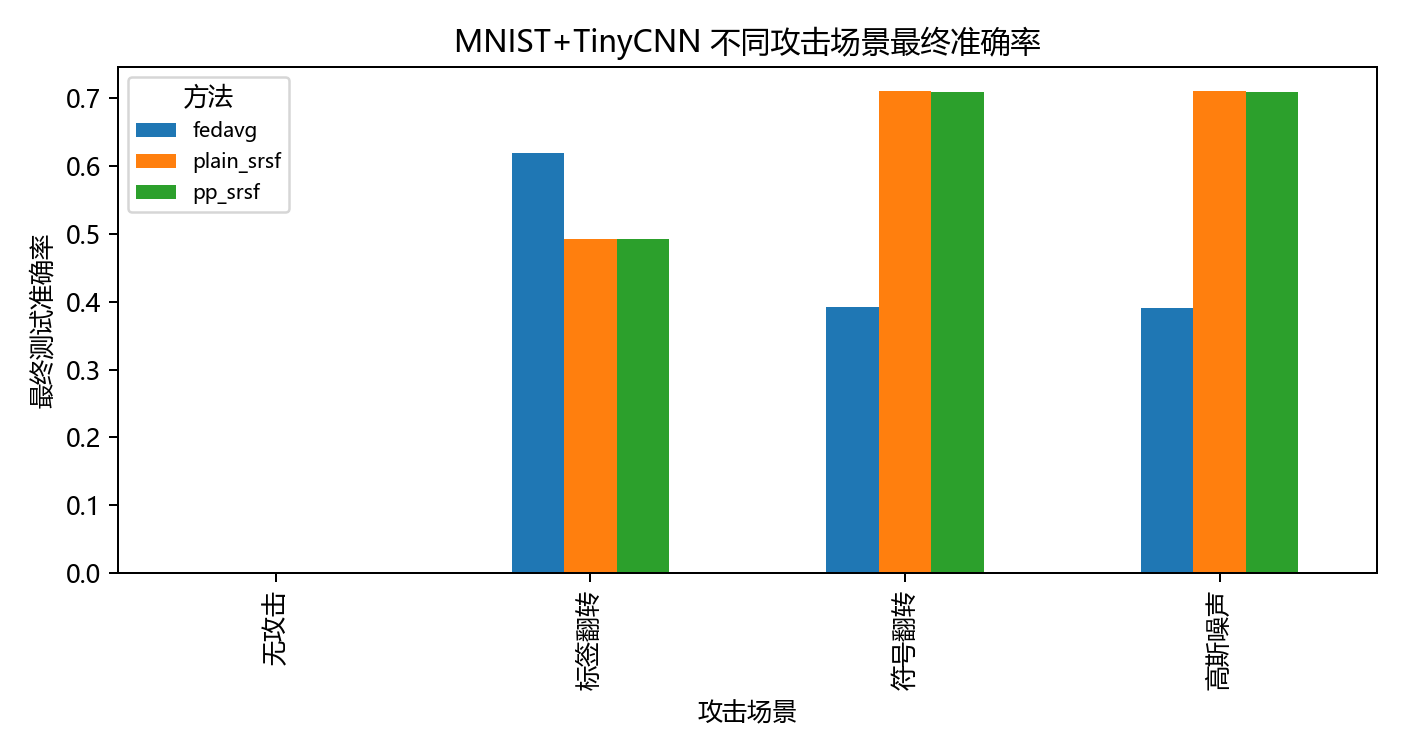
\includegraphics[width=0.86\linewidth]{../outputs/figures/attack_accuracy_grouped.png}
\caption{MNIST+TinyCNN 20 轮实验在不同攻击场景下的最终准确率}{}
\label{fig:attack-accuracy}
\end{figure}

\begin{figure}
\centering
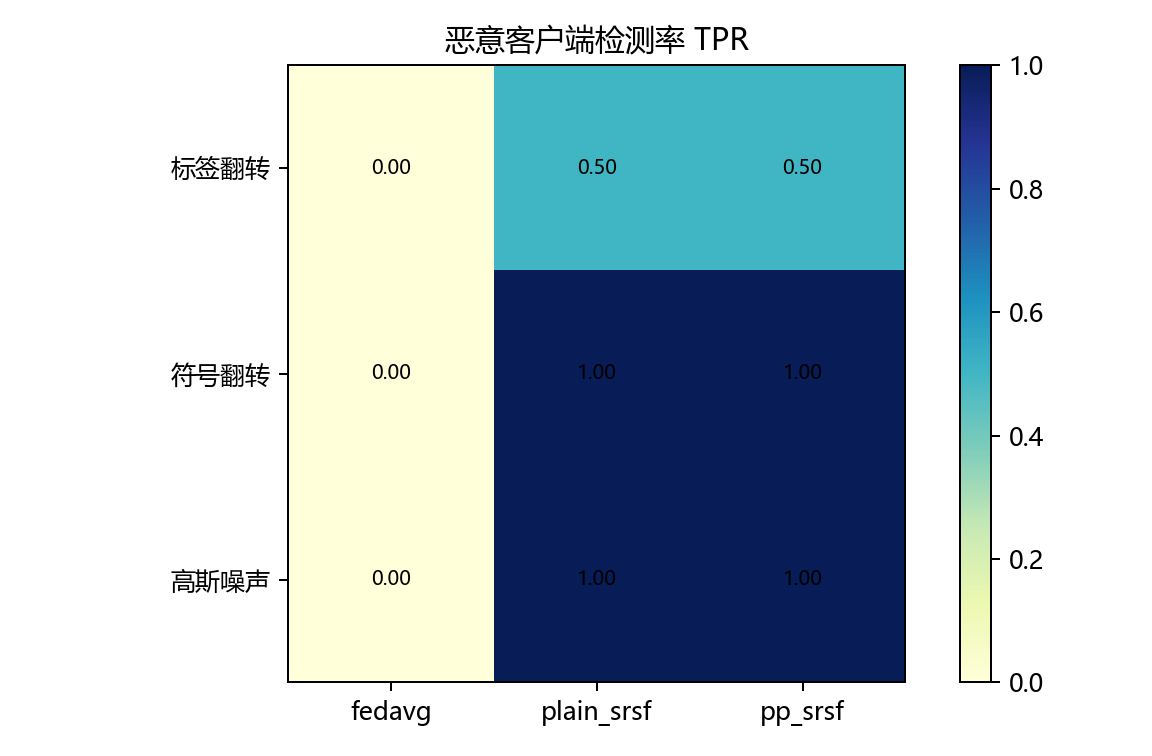
\includegraphics[width=0.72\linewidth]{../outputs/figures/detection_heatmap.png}
\caption{20\% 恶意客户端比例下不同方法的恶意客户端检测率}{}
\label{fig:detection-heatmap}
\end{figure}

\begin{figure}
\centering
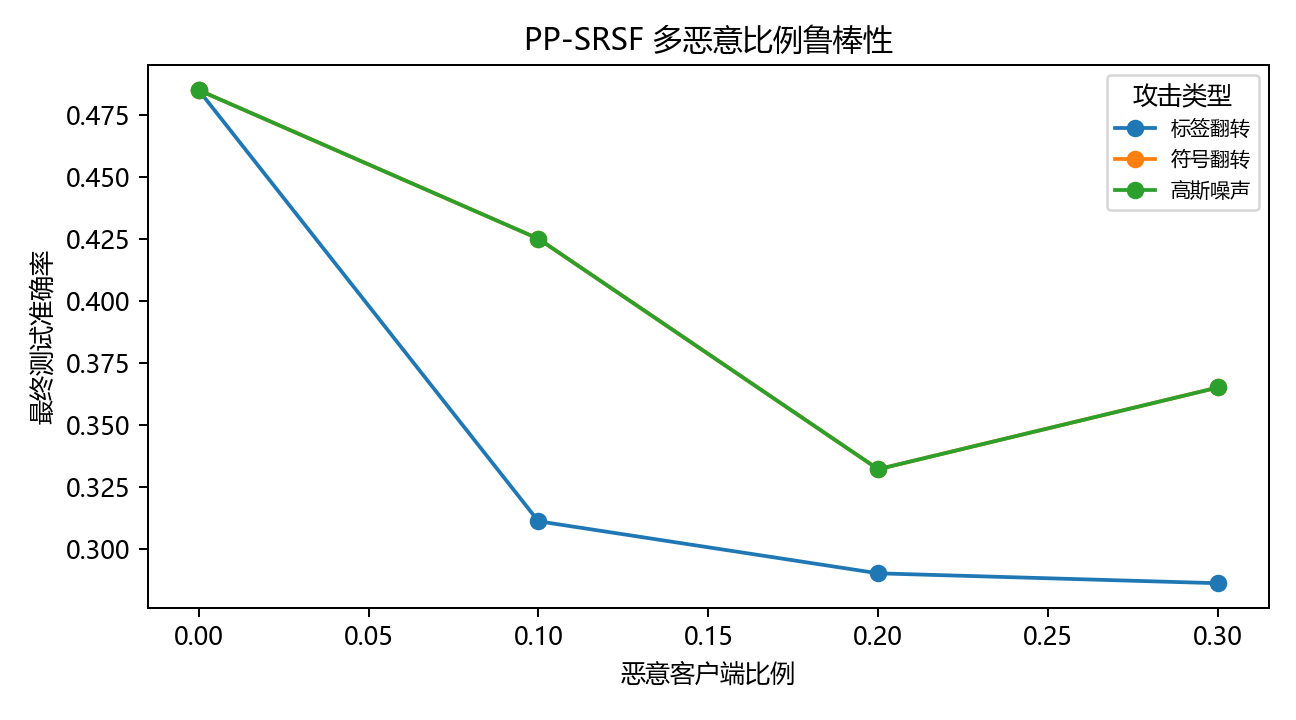
\includegraphics[width=0.82\linewidth]{../outputs/figures/pp_srsf_accuracy_vs_malicious_ratio.png}
\caption{不同恶意客户端比例下 PP-SRSF 的最终准确率}{}
\label{fig:pp-ratio}
\end{figure}

\subsection{多恶意比例与跨数据集讨论}
图\ref{fig:pp-ratio} 给出了 PP-SRSF 在不同恶意客户端比例下的准确率变化趋势。多比例实验的意义在于观察方法是否只在固定 $20\%$ 恶意客户端比例下偶然有效，还是能随攻击强度变化呈现合理响应。总体来看，无攻击或低恶意比例下 PP-SRSF 可以维持较稳定的模型性能；当恶意比例升高到 0.3 左右时，符号翻转和高斯噪声攻击仍能通过草图距离过滤得到一定控制，但标签翻转的波动更明显。这与前文分析一致：强离群攻击的异常性随恶意比例增加仍然可见，而隐蔽标签投毒更依赖数据分布和过滤阈值。

Fashion-MNIST 六轮单种子实验用于检验跨数据集、跨攻击趋势，表\ref{tab:fashion-strength} 给出最终轮结果。无攻击时 FedAvg 与 PP-SRSF 均为 0.382；在 $\rho=0.2$ 的符号翻转和高斯噪声下，PP-SRSF 分别达到 0.359 和 0.358，且 TPR 为 1.00、FPR 为 0；标签翻转下则降至 0.184。该结果再次显示强离群攻击易检测，而标签翻转会导致误杀。

\begin{table}
\centering
\caption{Fashion-MNIST+TinyCNN 六轮补充实验最终结果}{}
\label{tab:fashion-strength}
\begin{tabular}{lcccc}
\toprule
攻击（$\rho=0.2$） & FedAvg 准确率 & PP-SRSF 准确率 & TPR & FPR\\
\midrule
标签翻转 & 0.248 & 0.184 & 0.00 & 0.25\\
符号翻转 & 0.104 & 0.359 & 1.00 & 0.00\\
高斯噪声 & 0.161 & 0.358 & 1.00 & 0.00\\
\bottomrule
\end{tabular}
\end{table}

为降低单种子和六轮训练带来的偶然性，表\ref{tab:fashion-multiseed} 进一步给出标签翻转下 10 轮三种子复核。FedGT-$\hat n_m$ 的准确率和 Macro-F1 最高，但 FPR 也达到 0.208；PP-SRSF 的 TPR 为 0.833、FPR 为 0.042，最终准确率却只略高于 FedAvg。检测率与任务性能并非一一对应，Non-IID 少数类客户端的误杀会抵消过滤收益。

\begin{table}
\centering
\caption{Fashion-MNIST 标签翻转下三随机种子最终结果}{}
\label{tab:fashion-multiseed}
\begin{tabular}{lcccc}
\toprule
方法 & 准确率 & Macro-F1 & TPR & FPR\\
\midrule
FedAvg & $0.412\pm0.044$ & $0.320\pm0.061$ & 0.000 & 0.000\\
PP-SRSF & $0.416\pm0.061$ & $0.327\pm0.071$ & 0.833 & 0.042\\
PP-SRSF+Trust & $0.451\pm0.028$ & $0.353\pm0.043$ & 0.500 & 0.125\\
FedGT-$\hat n_m$ & $0.500\pm0.016$ & $0.423\pm0.017$ & 0.500 & 0.208\\
\bottomrule
\end{tabular}
\end{table}

\subsection{标签翻转增强与 Trust 扩展实验}
图\ref{fig:advanced-label-flip} 比较三种标签翻转变体。普通标签翻转下，FedAvg、PP-SRSF、Trust 与 FedGT-Ridge 的最终准确率依次为 0.580、0.473、0.593、0.617；all-to-one 下 PP-SRSF 与 Trust 达到 0.644 和 0.614，优于 FedAvg 的 0.481；pairwise 下距离方法降至 0.316 和 0.272，而 FedGT-Ridge 为 0.599。可见公共验证和组测试信号能补充距离统计，但没有一种过滤器在所有标签映射下占优。

\begin{figure}
\centering
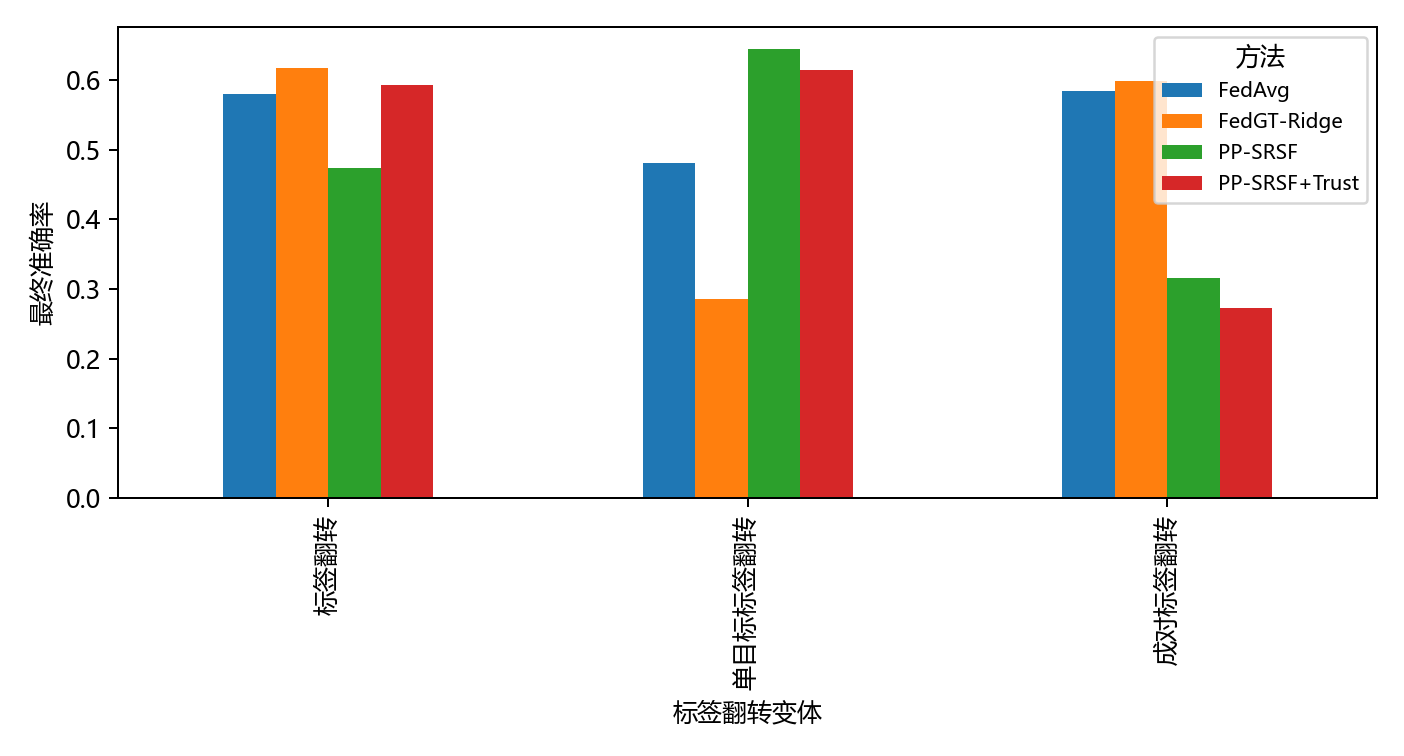
\includegraphics[width=0.82\linewidth]{../outputs/figures/advanced_label_flip_accuracy.png}
\caption{标签翻转增强实验下不同方法的最终准确率}{}
\label{fig:advanced-label-flip}
\end{figure}

\subsection{草图维度与多随机种子分析}
图\ref{fig:advanced-sketch} 给出符号翻转下三随机种子消融。PP-SRSF 从 $m=8$ 的 $0.674\pm0.104$ 上升到 $m=32$ 的 $0.694\pm0.076$，之后基本饱和；在线通信量从 12.0 KiB 增至 180.7 KiB，说明 $m=32$ 是较合适的精度--通信折中。图\ref{fig:advanced-seed} 显示普通标签翻转下 FedAvg、PP-SRSF、Trust、FedGT-Ridge 与 FedGT-$\hat n_m$ 的三种子结果分别为 $0.595\pm0.043$、$0.602\pm0.058$、$0.611\pm0.077$、$0.659\pm0.063$ 与 $0.662\pm0.079$。两种组测试解码结果接近，支持近期基线结论并非岭回归代理独有；但 FedGT-$\hat n_m$ 的 FPR 为 0.250，也暴露了 Non-IID 下聚类测试的误报代价。

\begin{figure}
\centering
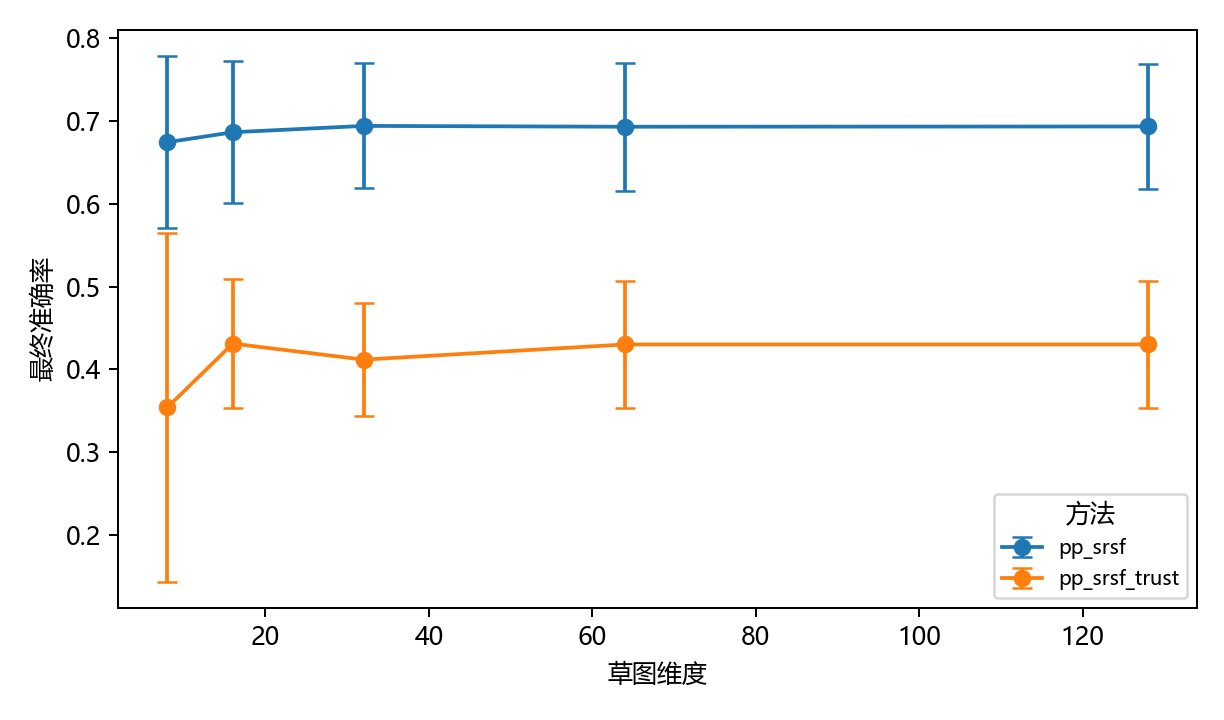
\includegraphics[width=0.78\linewidth]{../outputs/figures/advanced_sketch_dim_ablation.png}
\caption{不同草图维度下 PP-SRSF 与 PP-SRSF+History/Trust 的消融结果}{}
\label{fig:advanced-sketch}
\end{figure}

\begin{figure}
\centering
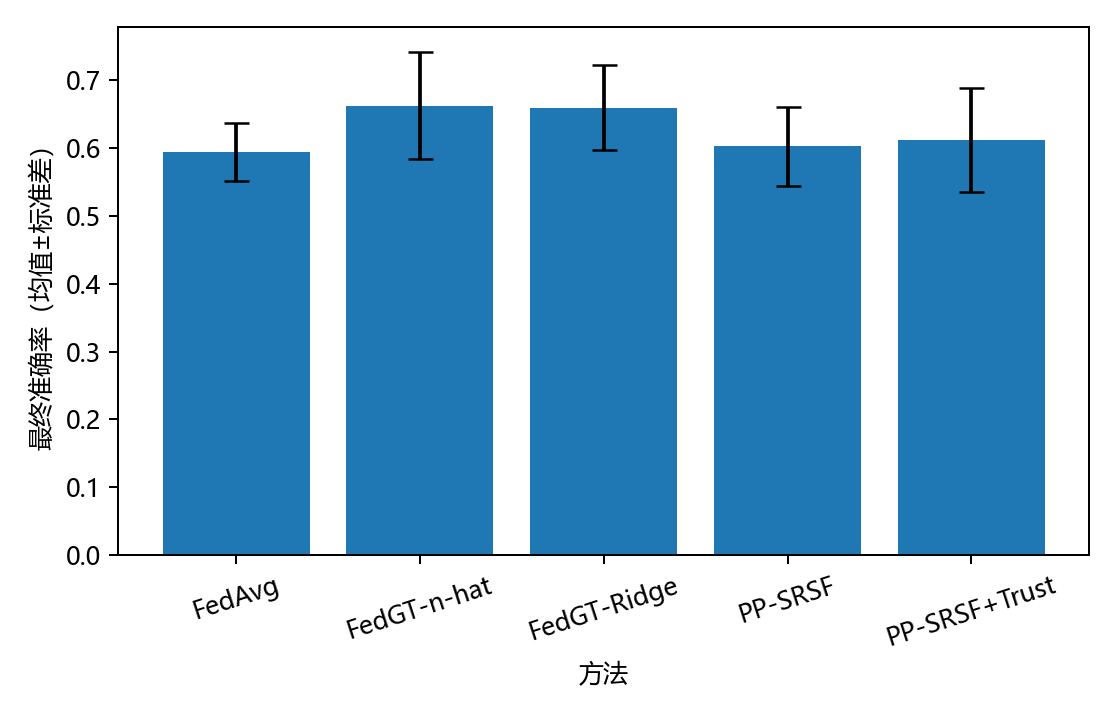
\includegraphics[width=0.72\linewidth]{../outputs/figures/advanced_seed_accuracy_mean_std.png}
\caption{三随机种子下标签翻转实验的准确率均值与标准差}{}
\label{fig:advanced-seed}
\end{figure}

\subsection{多数恶意压力测试}
图\ref{fig:advanced-majority} 同时报告准确率与检测率。符号翻转比例从 0.4 增至 0.6 时，PP-SRSF 的准确率为 0.684、0.694、0.709，TPR 均为 1.0；强反向更新即使数量占优，仍与诚实更新形成明显分离。标签翻转则相反：PP-SRSF 在 $\rho=0.4,0.5,0.6$ 时降至 0.340、0.112、0.018，而 FedGT-Ridge 为 0.593、0.573、0.391。攻击可分性比客户端计数更关键；当前方案仍未实现题目设想的密文几何中位数强保证。

\begin{figure}
\centering
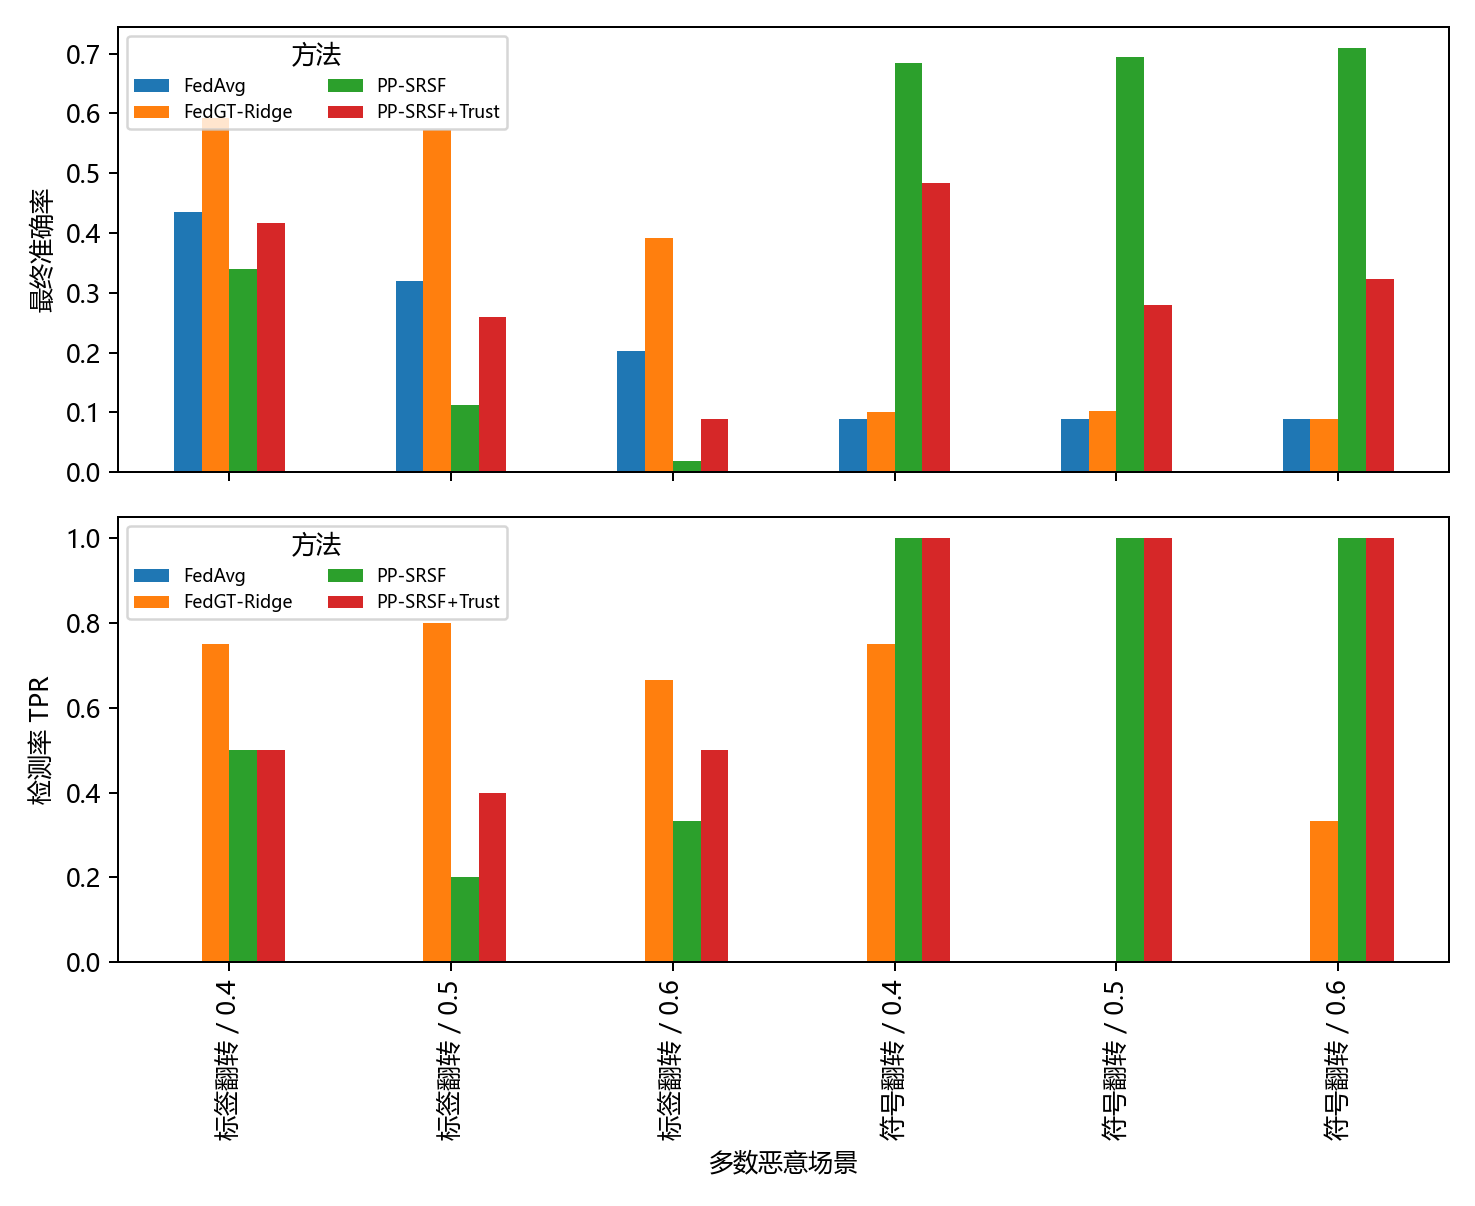
\includegraphics[width=0.82\linewidth]{../outputs/figures/advanced_majority_detection.png}
\caption{多数恶意比例下不同方法的最终准确率与检测率}{}
\label{fig:advanced-majority}
\end{figure}

\subsection{开销与可用性讨论}
PP-SRSF 的额外成本来自随机投影、草图份额传输和 Beaver 距离乘法。图\ref{fig:secure-distance-scaling} 给出十次重复的单进程协议微基准。$n=10,m=32$ 时，45 个客户端对共执行 1440 次安全乘法，耗时 $5.77\pm0.44$ ms，在线与离线通信分别为 45.7 KiB 和 67.5 KiB；$n=20,m=128$ 时耗时 $48.78\pm2.11$ ms、在线通信约 763.0 KiB。结果与 $O(n^2m)$ 分析一致。

\begin{figure}
\centering
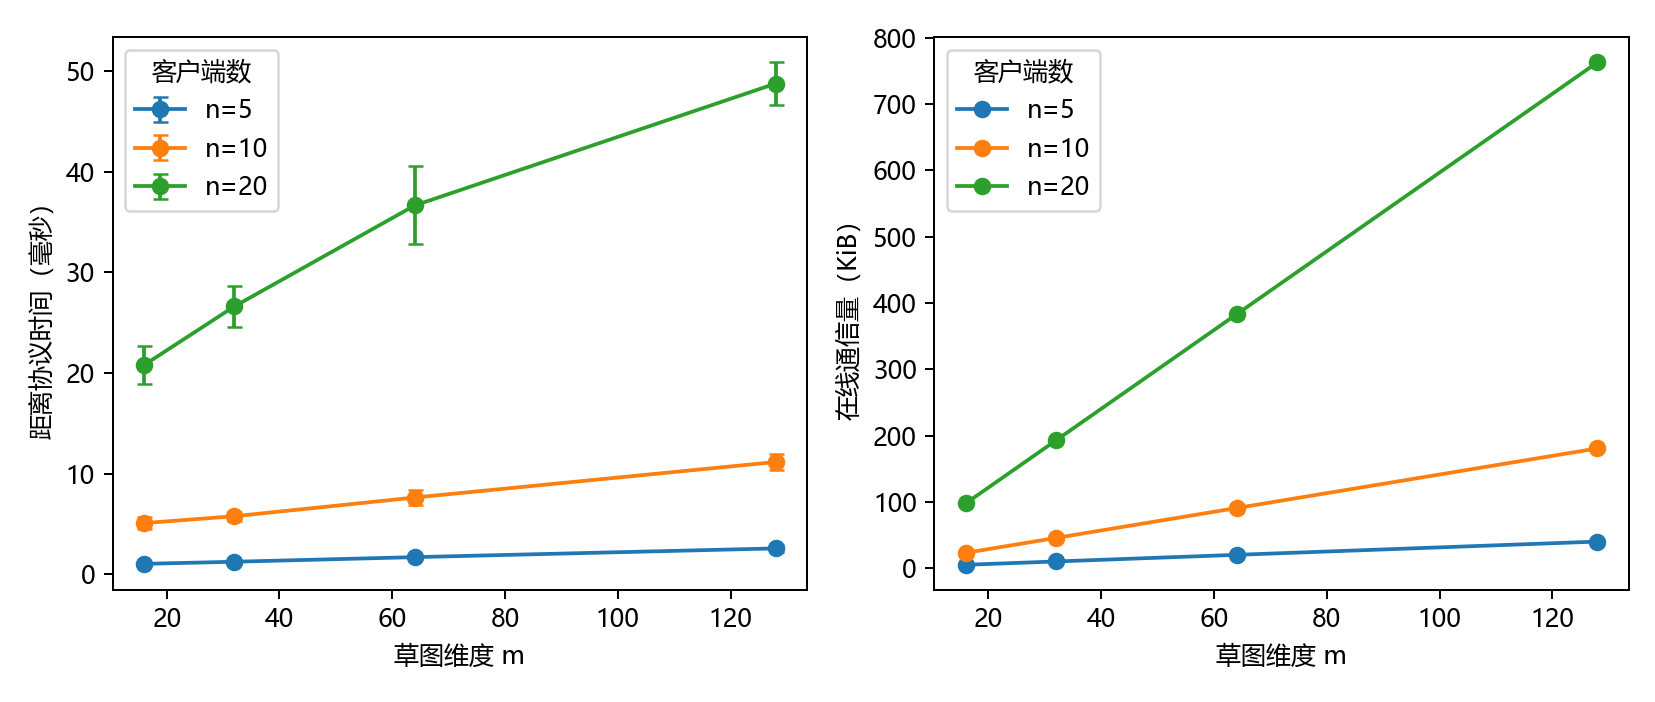
\includegraphics[width=0.95\linewidth]{../outputs/figures/secure_distance_scaling.png}
\caption{Beaver 草图距离协议随客户端数和草图维度的缩放结果}{}
\label{fig:secure-distance-scaling}
\end{figure}

该微基准仍不等价于真实跨网络 MPC：它计入本地有限域运算，并按公开份额数估计通信，但没有注入网络往返时延、序列化、认证和掉线恢复成本。因此结论限于协议缩放趋势，而非生产吞吐率。

\section{局限性与改进方向}
当前实现仍是课程原型，主要局限包括：
\begin{enumerate}[leftmargin=2em]
  \item 距离计算已使用 Beaver triple 份额乘法，但 triple 由可信预处理模拟生成，尚无认证份额和恶意安全保证。
  \item 安全聚合是简化掩码抵消机制，未处理真实移动 FL 中的 dropout。
  \item 几何中位数仍未在密文域实现，多数标签投毒下不能提供强鲁棒保证。
  \item 实验仍是 10--20 个客户端的小规模设置，需扩展 CIFAR-10、更深模型和更多种子。
  \item 标签翻转攻击的检测效果依赖攻击强度、数据异构程度和训练阶段。未来可引入跨轮动量、损失趋势或可信验证集信号，与草图距离共同构成复合异常分数。
\end{enumerate}

第一，密码协议仍需从半诚实 Beaver 原型推进到可证明的恶意安全协议。未来应引入分布式 triple 生成、消息认证码、承诺或零知识证明，保证聚合方无法篡改中间结果，客户端也无法提交与模型更新不一致的草图。

第二，安全聚合与鲁棒过滤之间的接口还比较粗糙。当前流程先用草图决定保留集合，再对保留客户端执行简化安全聚合；真实联邦学习还会遇到掉线、迟到和参与集合变化。未来 PP-SRSF 需要与 dropout-resilient SecAgg 结合，使被过滤客户端、主动掉线客户端和网络故障客户端在协议上可以区分处理\cite{bonawitz2017secagg}。

第三，鲁棒统计规则仍有改进空间。Krum 风格距离分数适合处理离群方向明显的攻击，但对标签翻转、后门植入和自适应投毒不够稳定。未来可以把单轮草图距离扩展为多信号评分，包括跨轮方向一致性、历史可信度、范数裁剪、公共验证集损失变化和多草图一致性。Aion 等工作也说明，输入检查和多轮协议效率同样会影响真实系统鲁棒性\cite{aion2025}。

第四，实验规模和统计显著性仍需增强。当前已覆盖两数据集、三随机种子、FedGT-Ridge 与精确枚举 LLR 的 FedGT-$\hat n_m$ 适配基线，以及 60\% 恶意比例；但仍未采用原文 BCH 矩阵、指定网络结构和官方完整流水线，后续应扩大客户端数量并加入 CIFAR-10。

第五，随机投影草图本身也存在隐私与鲁棒性的参数权衡。草图维度越大，距离保真度越高，但相似性泄露和通信开销也越大；草图维度越小，隐私和效率更好，但可能无法区分恶意更新与 Non-IID 诚实更新。未来可系统研究 $m$、量化尺度 $S$、模数 $p$、客户端数量 $n$ 和恶意比例 $\rho$ 之间的关系，并尝试多组低维草图投票。

总体而言，PP-SRSF 展示了秘密共享服务于联邦学习鲁棒过滤的可运行折中，但还不是完整工业级协议。后续应同时补强密码协议证明和更大规模机器学习实验。

\section{结论}
本文提出 PP-SRSF，将随机投影草图、Beaver 秘密共享距离和成对掩码聚合结合起来。实验表明，该方法对强离群拜占庭更新有效，$m=32$ 已取得较好的精度--通信折中；公共验证与组测试信号能缓解部分标签翻转，但多数隐蔽投毒仍是主要边界。未来工作将重点完善恶意安全 MPC、dropout-resilient SecAgg、密文几何中位数和更大规模实验。

\bibliographystyle{plain}
\bibliography{references}

\end{document}
